\section{A Global Estimate for Circumgalactic Absorption of Ionizing Radiation}
\label{escape}

The ionizing escape fraction from galaxies is an important parameter in models of reionization. Typically, one thinks about the escape fraction as a property of individual galaxies, determined by the absorption of ionizing radiation on small scales in the ISM. However it is interesting to ask whether there is significant absorption in the denser Circumgalactic Medium (CGM) surrounding galaxies. If we write the total escape fraction as the product of escape fractions, then $f_{esc}=f_{esc}(ISM)f_{esc}(CGM)$.  Here we use our simulation to derive an estimate of the globally averaged escape fraction as a function of redshift  due to the circumgalactic medium $\bar{f}_{esc}(CGM)$. 

Recall from Sec. \S\ref{Method} that the halo escape fraction is not a model input parameter, but is rather an ouput since the equation of radiative transfer is solved throughout the computational domain. Our halos are not well resolved internally, and so we are underestimating the amount absorption of ionizing radiation on galaxy ISM scales. However if significant absorption  occurs on scales of the virial radius or larger, then that would be simulated reasonably accurately. In the following we assume this is the case, and present results that can be taken to be an upper limit on the total escape fraction (ISM+CGM). 

Rather than measure the escape fraction halo by halo and take the average over all halos, we use a simpler method. Since we know every ionization requires an ionizing photon, and we have the ionization rate density as a field defined at every grid cell, then we can estimate $\bar{f}_{esc}(CGM)$ as follows (hereafter we drop the CGM modifier with the reader's understanding that this is what we are estimating):
\begin{equation}
\bar{f}_{esc}(I_t) = \int_{V_t}  n_\mathrm{H\,I}\Gamma_\mathrm{H\,I}^{ph} d^3x \bigg / \int_{V}  n_\mathrm{H\,I}\Gamma_\mathrm{H\,I}^{ph} d^3x  ,
\label{eq:fesc}
\end{equation}
\\where $\Gamma_\mathrm{H\,I}^{ph}$ is evaluated cell by cell via Equation \eqref{eq:photoionization}, $V$ is the simulation volume and $V_t$ denotes the integration includes only cells which satisfy $\Delta_b < 100.$ In other words, $\bar{f}_{esc}$ is the ratio of the number of ionizations in the IGM, as defined by the overdensity threshold, to the total number of ionizations in the volume. The modifier $I_t$ refers to this method of estimating $\bar{f}_{esc}$ (a superior method is presented below).



\begin{figure}
	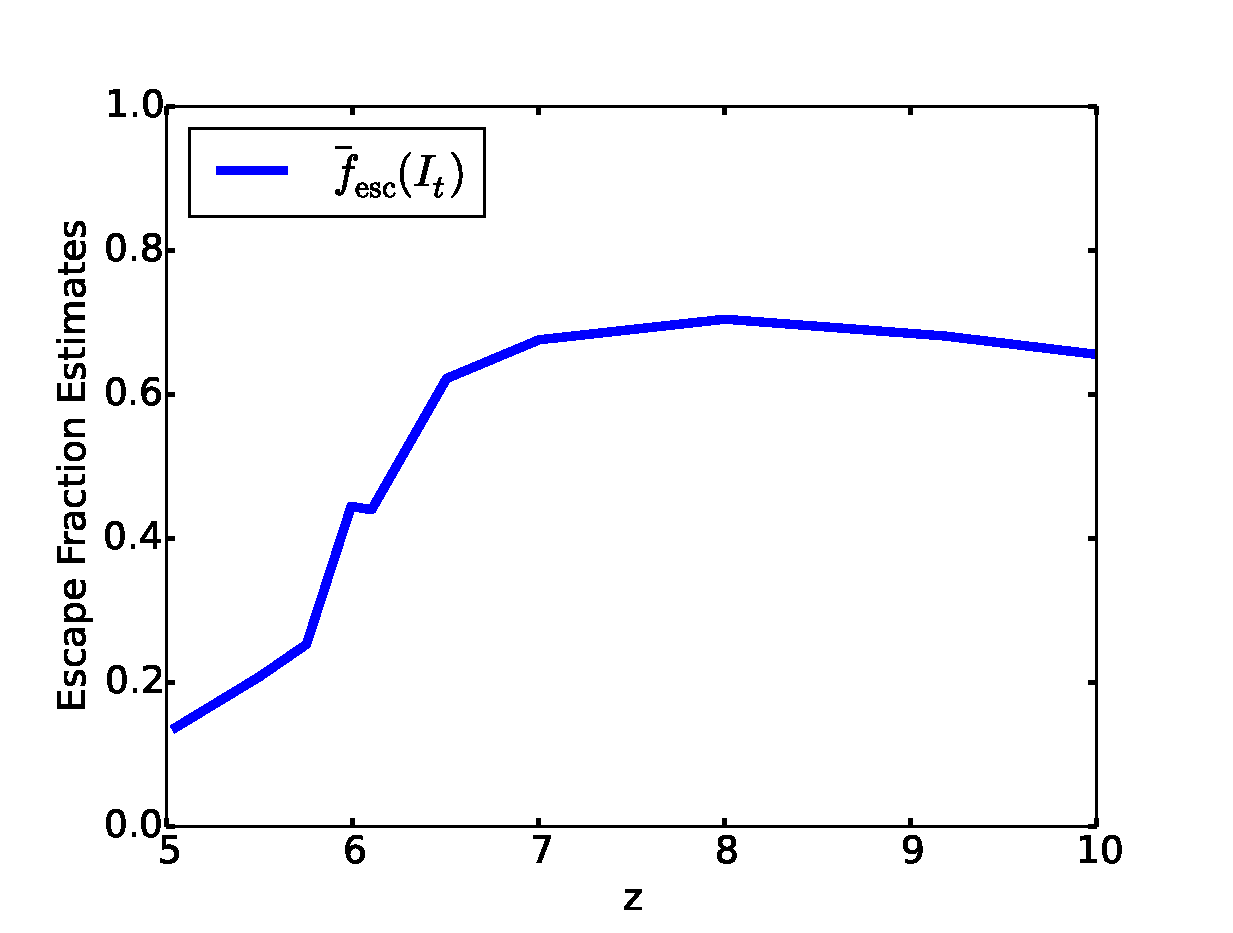
\includegraphics[width=0.5\textwidth]{EscFraction.eps}
	\caption{Estimate of the globally averaged ionizing radiation escape fraction due to circumgalactic absorption $\bar{f}_{esc}(I_t)$ computed as the ratio of the volume integrated ionization rate in the IGM ($\Delta_b < 100$) divided by the total ionization rate (Eq. \eqref{eq:fesc}). }
	\label{EscFraction}
\end{figure}

\begin{figure}
	\includegraphics[width=0.5\textwidth]{sanity_check_ratedensity.eps}
	\caption{Evolution of the volume averaged rate densities for: (1) ionizing photons injected into the IGM ($\dot{N}_\mathrm{IGM}$), (2) gas photoionization ($\dot{N}_t$), and (3) gas recombination  ($\dot{R}_t$) integrated over the singly thresholded volume $V_t$ defined as $\Delta_b<100$. The ionization rate density curve tracks the photon injection rate density curve in the photon starved regime at high redshifts, but begins to fall below it as the globally averaged ionization parameter approaches unity (Fig. \ref{IP}). After overlap, in the photon abundant regime, the ionization rate density is $\sim 20\times$ the photon injection rate density, but comes into balance with the recombination rate density.}
	\label{sanitycheckrate}
\end{figure}

The result is plotted in Fig. \ref{EscFraction}.  At high redshifts the escape fraction is high and relatively constant at $\bar{f}_{esc} \sim 0.65-0.7$. As overlap is approached $\bar{f}_{esc}$ drops considerably, reaching values of $\sim 0.2$ by $z=5.$ There is no obvious reason why the escape fraction should drop so dramatically at the epoch of overlap. To investigate this properly would require a statisical analysis of individual halo escape fractions, which we defer to a subsequent paper. Perhaps this is an artifact of how we are estimating $\bar{f}_{esc}$. While it is true that every ionization requires and ionizing photon in the photon starved regime (i.e., before overlap), after overlap the volume becomes optically thin to ionizing radiation, and it is not true that every ionizing photon causes an ionization in the box. This is illustrated in Fig. \ref{sanitycheckrate}. 

%The blue dashed line in Fig. \ref{sanitycheckrate} is $\dot{N}_{IGM}$ defined as $\bar{f}_{esc}\dot{N}_{sim}$. 
The curve labeled $\dot{N}_t$ is the actual ionization rate density measured in the simulation averaged over the entire 20 Mpc cubic volume satisfying the overdensity threshold $\Delta_b < 100$; i.e. precisely the numerator of Eq. \eqref{eq:fesc} divided by 20$^3$. The curve labeled $\dot{R}_t$ is the recombination rate density averaged over the same volume; i.e.
\begin{equation}
\dot{R}_t = \int_{V_t}  n_e n_\mathrm{H\,II}\alpha_B(T) d^3x  .
\label{eq:totrecombst}
\end{equation}

We see that ionization rate density $\dot{N}_t$ grows with redshift and reaches a maximum at $z \approx 6.5$, and then drops by roughly 0.8 dex by overlap completion at $z=5.8$. It continues to decrease thereafter. The reason for this sudden drop is that after overlap there are very few neutral atoms left to ionize ($n_\mathrm{H\,I}/n_\mathrm{H} \sim 10^{-5}$).  
%After overlap the large disparity between the $\dot{N}_{IGM}$ and $\dot{N}_t$ curves can then be understood as saying that the IGM becomes photon abundant. 

This can be illustrated by considering the {\em global ionization parameter}, which is the number of ionizing photons per neutral H atom $\Gamma_{IP} = \langle n_{ph}\rangle/\langle n_{H I} \rangle$ averaged over the entire volume. Specifically, we integrate the grey radiation energy density divided by the mean photon energy $\bar{\epsilon}$ over the singly thresholded volume, and divide by the number of H {\footnotesize I} atoms in the same volume:
\begin{equation}
\Gamma_{IP} =  \int_{V_t}  (E/\bar{\epsilon}) d^3x \bigg / \int_{V_t}  n_{HI} d^3x. 
\label{eq:IP}
\end{equation}
We see from Fig. \ref{IP} that $\Gamma_{IP}$ grows from $\sim 10^{-3}$ at $z=10$ to unity at $z\approx 6.5$ just before overlap. Thereafter $\Gamma_{IP}$ grows very rapidly, reaching a value around $10^5$ at the overlap redshift, and leveling off at around $10^6$ below that.  From the standpoint of the global ionization parameter, reionization begins photon starved but completes photon abundant. 
  
\begin{figure}
	\includegraphics[width=0.5\textwidth]{Gamma.eps}
	\caption{Redshift evolution of the global ionization parameter as defined in Eq. \eqref{eq:IP}. }
	\label{IP}
\end{figure}

Returning to Fig. \ref{sanitycheckrate} we see that the recombination rate density $\dot{R}_t$ curve tracks the ionization rate density curve to $z\sim 7$, but is about 0.7 dex lower in magnitude, as it must be if the ionized volume filling fraction is to grow. As overlap is approached ionizations and recombinations come into balance, but the recombination rate density has dropped considerably since it reached its maximum value at $z \approx 6.5$. This is also the redshift at which the ionization rate achieves a maximum, and when the global ionization parameter reaches unity.  We also observe that the $f_{esc}$ curve in Fig. \ref{EscFraction} begins its precipitous drop at this redshift. We believe all of these events signal the rapid rise in the global ionization parameter below $z=6.5$, and not some change in the escape fraction of young galaxies. 

Counting the fraction of all ionizations occuring outside halos is not a reliable estimate of the escape fraction for $\Gamma_{IP} \gg 1$ because it does not count the photons in the radiation field that have nothing to ionize. Therefore we need to modify Eq. \eqref{eq:fesc} to include photons which build up of the radiation field: 
\begin{equation}
\bar{f}_{esc} = \int_{V_t}  (n_\mathrm{H\,I}\Gamma_\mathrm{H\,I}^{ph} + \frac{1}{\bar{\epsilon}}\frac{dE}{dt}) d^3x \bigg / \int_{V}  (\eta/\bar{\epsilon}) d^3x . 
\label{eq:fescimproved}
\end{equation}
\\Here the numerator is the rate at which ionizing photons are causing ionizations in the IGM and building up the UV background, and the denominator is volume integrated ionizing photon production rate. 

Fig. \ref{RadEscFraction} plots $\bar{f}_{esc}$ calculated according to Eq. \eqref{eq:fescimproved}. Each contribution to $\bar{f}_{esc}$ is plotted separately, as well as the sum. We see that $\bar{f}_{esc}$ is roughly constant with redshift with a value of around 0.6. We see that as the contribution due to ionizations declines below $z\sim 7$, the contribution due to the change in radiation background intensity increases in a compensating fashion. This confirms our earlier suspicions and gives us a better estimate of the mean circumgalactic attenuation of ionizing radiation from young galaxies. 

\begin{figure}
	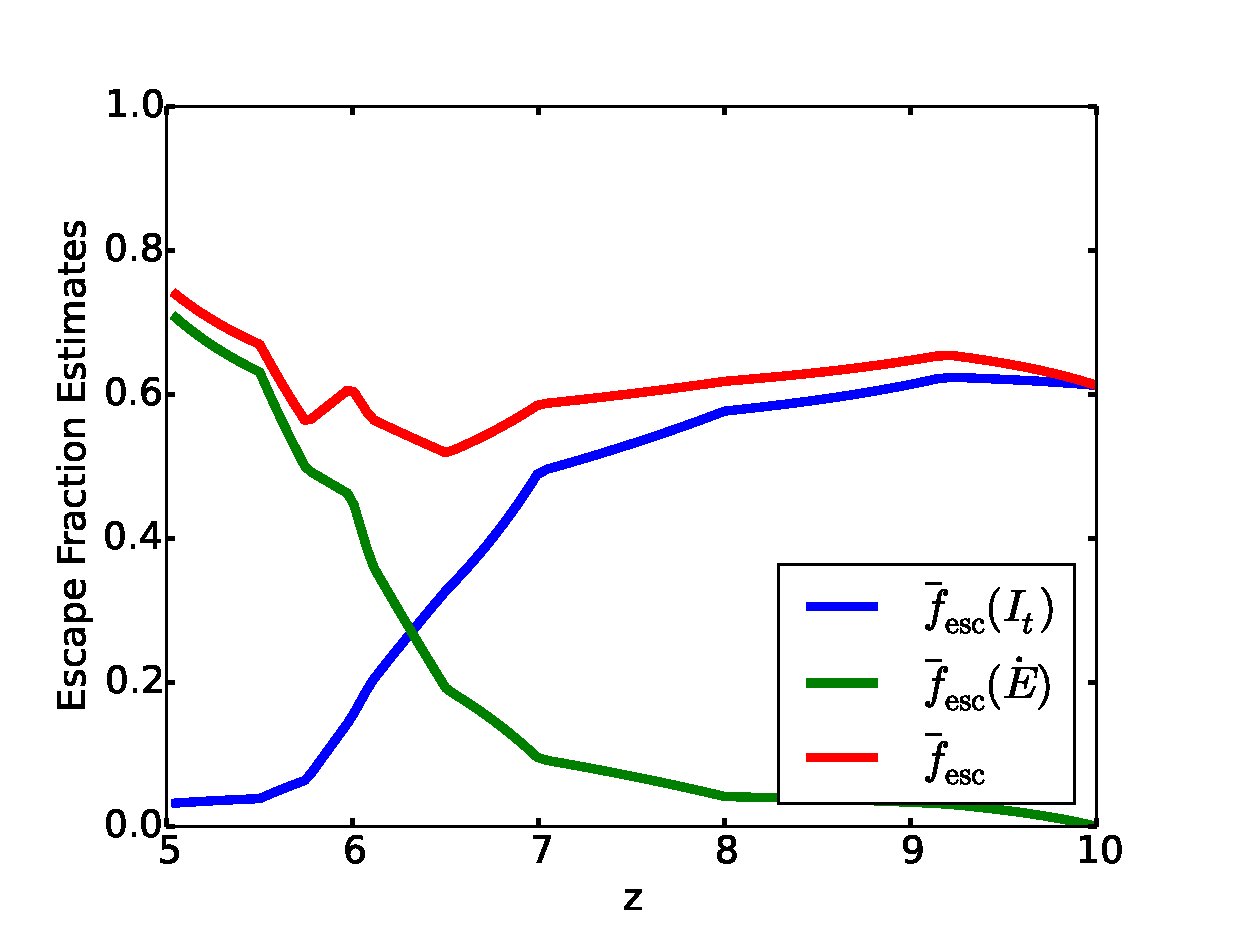
\includegraphics[width=0.5\textwidth]{RadEscFraction.eps}
	\caption{Redshift evolution of the globally averaged escape fraction contribution from circumgalactic absorption as estimated by the number of ionizations occuring in the IGM and the buildup of the ionizing radiation background. The curves labeled $\bar{f}_{esc}(I_t), \bar{f}_{esc}(\dot{E})$ plot the contributions of the first and second terms in Eq. \eqref{eq:fescimproved}, while the curve labeled $\bar{f}_{esc}$ plots their sum.}
	\label{RadEscFraction}
\end{figure}

To complete the picture we plot in Fig. \ref{sanitycheckrate} the number density of ionizing photons escaping into the IGM, calculated as $\dot{N}_{IGM}=\bar{f}_{esc}\dot{N}_{sim}$, where $\dot{N}_{sim}$ is the ionizing photon production rate in the simulation, and  $\bar{f}_{esc}$ is the improved estimate for the escape fraction calculated using Equation \eqref{eq:fescimproved}. We see that at high redshifts the $\dot{N}_{IGM}$ and $\dot{N}_t$ track each other closely. This tells us two things. First, that reionization at high redshifts when $Q_{\mathrm{H\,II}} \ll 1$ is photon starved, in the sense that every ionizing photon emitted results in an ionization. And second that our estimate of $\bar{f}_{esc}$ is reasonably accurate at these redshifts. However, as redshift decreases, the two curves systematically begin to deviate from one another in the sense that $\dot{N}_t < \dot{N}_{IGM}$. Beginning at $z = 6.5$ the ionization rate density begins to decrease while the ionizing photon production rate into the IGM continues to rise. 
After overlap the large disparity between the $\dot{N}_{IGM}$ and $\dot{N}_t$ curves can then be understood as saying that the IGM becomes photon abundant. 

The ratio of ionization rate density and the photon injection rate into the IGM is plotted in Fig. \ref{Ndot_Ratio}. The ratio is unity initially, and slowly decreases until $z\approx 7$, and then drops rapidly as overlap is approached. After overlap the ratio is about 0.05. In other words, after overlap, the photon production rate is about 20$\times$ the ionization rate in a volume averaged sense. Since the ionization and recombination rates are in balance after overlap, we conclude that the volume averaged photon injection rate is about 20$\times$ the recombination rate. 


\begin{figure}
	\includegraphics[width=0.5\textwidth]{Ndot_Ratio.eps}
	\caption{Ratio of the volume integrated photoionization rate in the IGM $\dot{N}_t$ to the integrated photon injection rate into the IGM $\dot{N}_{IGM}$, where the IGM is defined as cells with $\Delta_b < 100$. The ratio is near unity initilly, remains high until $z\approx 7$ ($Q_{HII} \approx 0.5$), and then drops rapidly as overlap is approached and the IGM becomes highly ionized.}
	\label{Ndot_Ratio}
\end{figure}



